\documentclass[14pt,dvipdfmx]{beamer}

\newcommand{\backupbegin}{
  \newcounter{framenumberappendix}
  \setcounter{framenumberappendix}{\value{framenumber}}
}
\newcommand{\backupend}{
  \addtocounter{framenumberappendix}{-\value{framenumber}}
  \addtocounter{framenumber}{\value{framenumberappendix}} 
}

\usetheme{Madrid}
\setbeamertemplate{navigation symbols}{}

\usepackage{graphicx}
\usepackage{amsmath}
\usepackage{amsfonts}
\usepackage{amssymb}
\usepackage{comment}
\usepackage{txfonts}
\usepackage{ascmac}
\usepackage{moreverb}
\usepackage{array,booktabs}


%\mathversion{bold}
\renewcommand{\familydefault}{\sfdefault}
\renewcommand{\kanjifamilydefault}{\gtdefault}
\renewcommand{\thefootnote}{\arabic{footnote}}
\setbeamerfont{title}{size=\large,series=\bfseries}
\setbeamerfont{frametitle}{size=\large,series=\bfseries}
\setbeamertemplate{frametitle}[default][center]
\usefonttheme{professionalfonts}
%
\newcommand{\bd}[1]{\mbox{\boldmath $#1$}}
\def\smskip{\par\vskip 5pt}
\def\QED{\hfill $\Box$ \smskip}
%
\title[研究発表]{関心度の高い他研究室の\\発表聴講可能性を高める\\特別研究報告審査会スケジュールの作成}
\author[大原源悠]{都$14-0033$ 大原源悠 \\ システム最適化研究室}
\institute[システム最適化研究室]{}
\date{February $15$, $2018$}

\begin{document}
%
\frame{\titlepage}
%

\frame{
  \frametitle{本研究の背景と目的}
  %
   \begin{beamerboxesrounded}[shadow=false]
    {背景}
    \begin{itemize}
    \item 若林\footnote[1]{若林祐麻 「特別研究報告審査会のスケジュール作成の自動化」\\ \quad(2016年度 都市システム工学科卒)}がスケジュール一覧表を自動で作成する\\インターフェースを作成
      \begin{itemize}
      \item ある教員から\\「研究内容が近い研究室の教員がお互いの研究室の\\発表を聞けるようにしたい」という要望を頂いた
      \item 現在のインターフェース:修正すべき事項多数あり 
      \end{itemize}
     \end{itemize}
   \end{beamerboxesrounded}
    \begin{beamerboxesrounded}[shadow=false]
    {目的}
    \begin{itemize}
    \item スケジュール作成問題の改良
    \item インターフェースの利便性向上
      \end{itemize}
   \end{beamerboxesrounded}

}

\frame{
  \frametitle{スケジュール作成問題の改良 $1/2$}
  \begin{itemize}
      \item 要望を実現するために新たな制約条件を追加した\\最適化モデルを作成
     \begin{itembox}[l]{頂いた要望}
      研究内容が近い研究室の教員が、お互いの\\研究室の発表を聞けるようにしたい
     \end{itembox}
     \end{itemize}
    \begin{itemize}
     \item 「関心度が高く発表を聞きに行きたい研究室同士の発表セッションが重複しない」という制約条件を追加
    \end{itemize}
  }

       
\frame{
  \frametitle{スケジュール作成問題の改良 $2/2$}
  \begin{itemize}
    \item 研究室$A$の教員が研究室$B$の学生の発表を\\聞きたいとき,発表セッションが同じだと,\\発表を聞けない可能性がある.
   \end{itemize}
  \begin{figure}[tpb]		
    \begin{center}	
      \includegraphics[scale=0.6]<1>{befor.PNG}
      \includegraphics[scale=0.6]<2>{af.PNG}
       \includegraphics[scale=0.35]<3>{siki.PNG}
    \end{center}
  \end{figure}
  %
}


\frame{
  \frametitle{制約条件}
  \begin{beamerboxesrounded}[shadow=false]{絶対制約}
    \begin{itemize}
    \item 全学生が $1$ 回ずつ発表する
    \item 学生は自分自身と研究室の教員が共に\\参加可能なセッションで発表する
    \item 各教員が司会をするのは$1$度までとする
    \end{itemize}
  \end{beamerboxesrounded}
  \begin{beamerboxesrounded}[shadow=false]{考慮制約}
    \begin{itemize}
    \item 各研究室は全ての時間帯で発表するのが\\望ましい
    \item 各研究室の中で,時間帯毎の発表者数の差は\\少ない状態が望ましい
    \item 同じセッションで発表するのが望ましい学生の\\組合せをできるだけ成立させる
    \end{itemize}
  \end{beamerboxesrounded}
  }
    

\frame{
  \frametitle{インターフェースの利便性向上 $1/2$}
  \begin{itemize}
  \item 研究室データを記入する Excel ファイルの\\記入方法が異なっていた
    \begin{itemize}
    \item 教員名を「姓+名」とする研究室と「姓+先生」と\\する研究室に分かれた
    \item 氏名の間に半角あるいは全角スペースを入れる研究室と入れない研究室に分かれた
    \item 学籍番号を半角入力する研究室と全角入力する研究室に分かれた
    \end{itemize}
  \item データの一部を手動で修正する必要があった
  \end{itemize}
   }

\frame{
  \frametitle{インターフェースの利便性向上 $2/2$}
  \begin{itemize}
  \item Excel ファイルへの記入方法を統一
    \begin{itemize}
    \item ドロップダウンメニューから選択するように変更
    \end{itemize}
  \end{itemize}
   \begin{figure}[tpb]		
    \begin{center}	
      \includegraphics[scale=0.5]<1>{int.PNG}
      \includegraphics[scale=0.6]<2>{int2.PNG}
    \end{center}
   \end{figure}
}


\frame{
  \frametitle{作成したスケジュール}
    \textcolor{red}{\textbullet} 海岸工学研究室と環境防災水工学研究室\\
    \textcolor{blue}{\textbullet} コンクリート工学研究室と複合材料構造研究室\\
    \textcolor{green}{\textbullet} 複合材料構造研究室 構造工学研究室\\
    \textcolor{yellow}{\textbullet} 複合材料構造研究室と鋼構造デザイン研究室\\
    \textcolor{magenta}{\textbullet} $OR$研究室社会システム研究室\\
    \textcolor{black}{\textbullet} $OR$研究室とシステム最適化研究室
  \begin{figure}[tpb]		
    \begin{center}	
      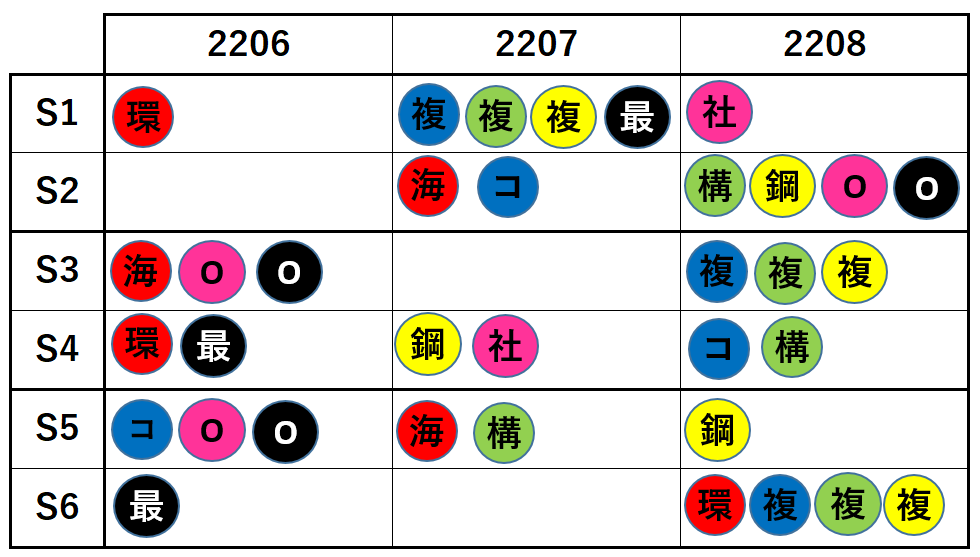
\includegraphics[scale=0.35]{g.PNG}
    \end{center}
  \end{figure}
}

\frame{
  \frametitle{まとめと課題}
  \begin{beamerboxesrounded}[shadow=false]
    {まとめ}
    \begin{itemize}
    \item スケジュール作成問題の改良
      \begin{itemize}
      \item 新たな制約条件を追加
      \item $2017$年度特別研究報告審査会スケジュールを作成
      \end{itemize}
    \item インターフェースの利便性向上
      \begin{itemize}
      \item Excel ファイルへの記入方法統一
      \end{itemize}
    \end{itemize}
  \end{beamerboxesrounded}
  \begin{beamerboxesrounded}[shadow=false]
    {今後の課題}
    \begin{itemize}
    \item 一部手動での修正が必要であった
      \begin{itemize}
      \item 制約条件の改良が必要
      \end{itemize}
    \item より「最適なスケジュール」の作成
    \end{itemize}
  \end{beamerboxesrounded}
}

\appendix
\backupbegin

\frame{
  \frametitle{スケジュール作成問題の定式化 ($1/3$)}
  \begin{beamerboxesrounded}[shadow=false]{絶対制約 ($1/2$)}
    \begin{itemize}
    \item 全学生が $1$ 回ずつ発表する
    \item 学生は自分自身と研究室の教員が共に\\参加可能なセッションで発表する
    \item 各研究室は複数のセッションで発表する
    \item 研究室が同じ学生は教室をまたいで同時刻の\\セッションで発表しない
    \item 学生個人の発表と,指定された研究室に所属する\\学生の発表が対応する
    \item 一体運用を行う研究室は同じセッションにて\\発表する
    \end{itemize}
  \end{beamerboxesrounded}
  %
}

\frame{
  \frametitle{スケジュール作成問題の定式化 ($2/3$)}
  \begin{beamerboxesrounded}[shadow=false]{絶対制約 ($2/2$)}
    \begin{itemize}
    \item 各セッションの発表人数の計算
    \item 各セッションの発表者数は上限を超えない
    \item 研究室の時間帯毎の発表者数の計算
    \item 全セッションで教員が司会をする
    \item 研究室での発表がある場合,(その研究室の)\\教員が司会をすることがある
    \item 各教員が司会をするのは $1$ 度までとする
    \end{itemize}
  \end{beamerboxesrounded}
  %
}

\frame{
  \frametitle{スケジュール作成問題の定式化 ($3/3$)}
  \begin{beamerboxesrounded}[shadow=false]{考慮制約}
    \begin{itemize}
    \item 同時刻に行われているセッションにおいて\\発表人数の最大と最小の差は $1$ 以下とするのが\\望ましい
    \item 各研究室は全ての時間帯で発表するのが\\望ましい
    \item 各研究室の中で,時間帯毎の発表者数の差は\\少ない状態が望ましい
    \item 同じセッションで発表するのが望ましい学生の\\組合せをできるだけ成立させる
    \end{itemize}
  \end{beamerboxesrounded}
  %
}

\frame{
  \frametitle{モデル$1$}
    %
  \begin{itemize}
  \item 研究室Aの教員が研究室Bの学生の発表を\\   聞きたいときに、発表順序を考慮すると\\教室の移動が可能な場合がある
  \end{itemize}
  \begin{figure}[tpb]		
    \begin{center}	
      \includegraphics[scale=0.5]<1>{BeforeOrder.PNG}
      \includegraphics[scale=0.5]<2>{AfterOrder.PNG}
    \end{center}
  \end{figure}
  %
}

\frame{
  \frametitle{間違いがあった制約条件}
   \begin{figure}[tpb]		
    \begin{center}	
      \includegraphics[scale=0.4]<1>{k3.PNG}
    \end{center}
  \end{figure}
}



\backupend


\end{document}
%%%%% End of file %%%%%
